\section{Generative Adversarial Networks}

  To introduce this topic, let's go back to the fundamentals talk about what the goal of modeling in general is. There exists in the real world a true distribution of the data we're interested in, and a generative model attempts to copy this distribution so that we can generate new synthetic observations. That is, density estimation really boils down to making sure that 
  \[\mathbb{P}_{\mathrm{observations}} \approx \mathbb{P}_{\mathrm{synthetic obs.}}\]
  \begin{center}
    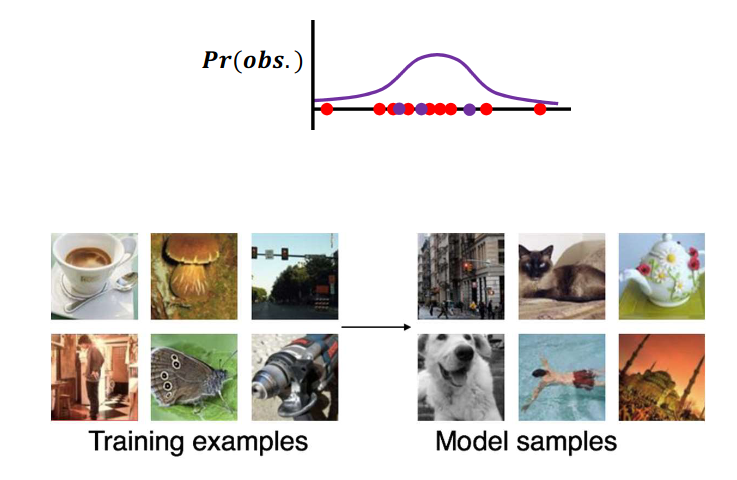
\includegraphics[scale=0.4]{img/09_GAN/training_vs_model_samples.png} 
  \end{center}
  The simplest types of densities can be analytically written and can be sampled from directly (e.g. Gaussian with inverse CDF or Box-Muller transform). More complicated models such as the RBM and VAE cannot be analytically written, but can still be directly sampled from with probabilities. GANs are implicit in the way that you can't estimate the probabilities but you can still sample from them. You essentially want to take some simple latent distribution and construct a differentiable a \textbf{Generator model} that maps it to a more complicated distribution in the observable space. 
  \begin{center}
    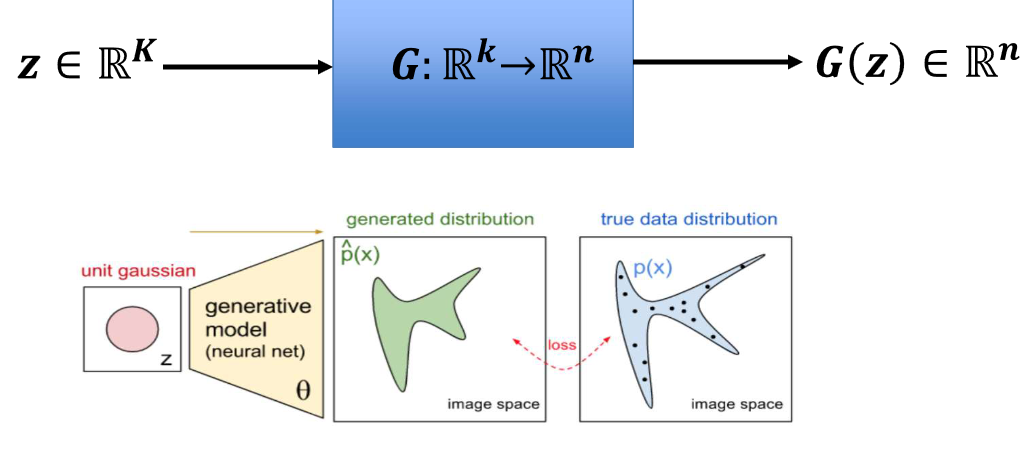
\includegraphics[scale=0.4]{img/09_GAN/implicit_gen_models.png}
  \end{center} 

  The problem with VAEs is that they tend to generate blurry images, which is the result of optimizing a variational lower bound rather than the true objective. This makes it easy to identify whether a given image is from the true dataset or has been artifically generated. In contrast, GANs generate high-resolution images by optimizing a pair of generator and disciminator neural networks, which play a game where one tries to bea the other. 
  \begin{enumerate} 
    \item The \textbf{generator} tries to generate fake samples to fool the discriminator. We sample from a latent space $\mathbf{z}$ and run that through the neural network to get $\mathbf{x} = \mathcal{G}_{\theta_g} (\mathbf{z})$.i It should be differentiable, but does not have to be invertible.   
    \item The \textbf{discriminator} tries to distinguish between real and fake samples, like a critic which can tell from real from fake. It should also be differentiable, and its output is essentially $0 \leq \mathcal{D}_{\theta_d}(\mathbf{x}) \leq 1$, with a value of $1$ if real, $0$ if fake.  
  \end{enumerate}
  We want to train these two models against each other, and in the end, we throw $\mathcal{D}$ away, since it's only role is to force $\mathcal{G}_{\theta_g}$ to work harder, which leaves us with a really good generative $\mathcal{D}_{\theta_g}$. 
  \begin{center}
    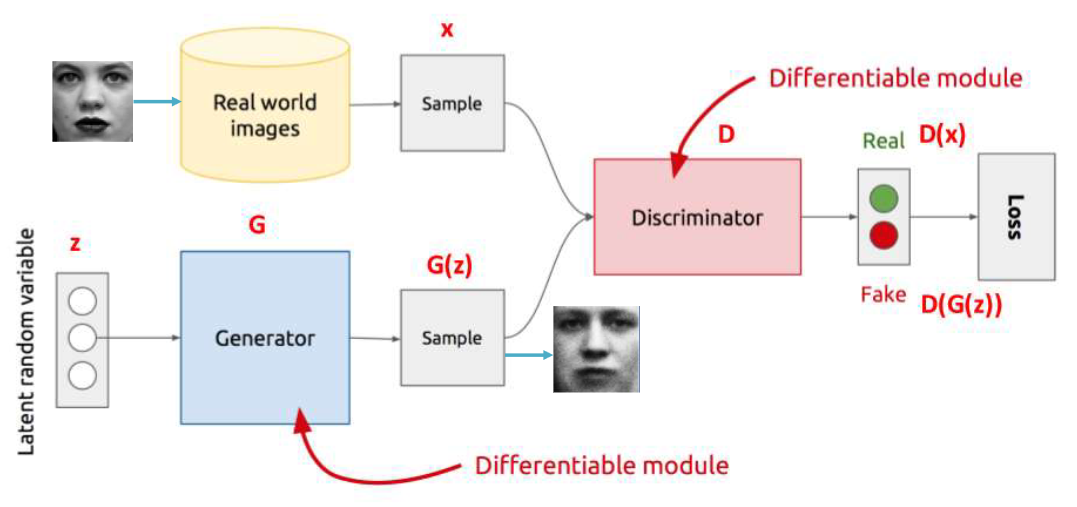
\includegraphics[scale=0.4]{img/09_GAN/general_gan_architecture.png}
  \end{center} 

  Now each of these networks will have its own set of parameters which we have to optimize. We want to optimize them by maximizing the likelihood such that the model says ``real" to the samples from the world and ``fake" to the generated samples. This leads to 
  \[\mathcal{L}(\theta_d, \theta_g) = V(\mathcal{D}, \mathcal{G}) = \underbrace{\mathbb{E}_{x \sim real} \big[ \log \mathcal{D}_{\theta_d}(\mathbf{x}) \big]}_{\substack{\text{log-prob that } \mathcal{D} \text{ correctly} \\ \text{predicts real data as real}}} + \underbrace{\mathbb{E}_{\mathbf{z}} \big[ \log \big( 1 - \mathcal{D}_{\theta_d} ( \mathcal{G}_{\theta_g} (\mathbf{z}))\big)\big]}_{\substack{{log-prob that } \mathcal{D} \text{ correctly} \\ \text{predicts generated data as fake} }}\]
  Therefore, the discrimiator is trying to maximize its reward (to get max value of $0$), and the generator is trying to minimize the disciminator's reward (pulling this log probability down to $-\infty$). This is known as a \textbf{minimax} optimization problem, and we have to find 
  \[\min_{\theta_g} \max_{\theta_d} V(\mathcal{D}_{\theta_d}, \mathcal{G}_{\theta_g})\]
  which is some saddle point. Note that the generator has no effect on the probability of $\mathcal{D}$ correctly identifying real images, so it only focuses on the latter term. The idea is to train both models simultaneously via SGD using mini-batches consisting of some generated samples and some real-world samples, which is called the \textbf{alternative gradient descent algorithm}.  
  \begin{center}
      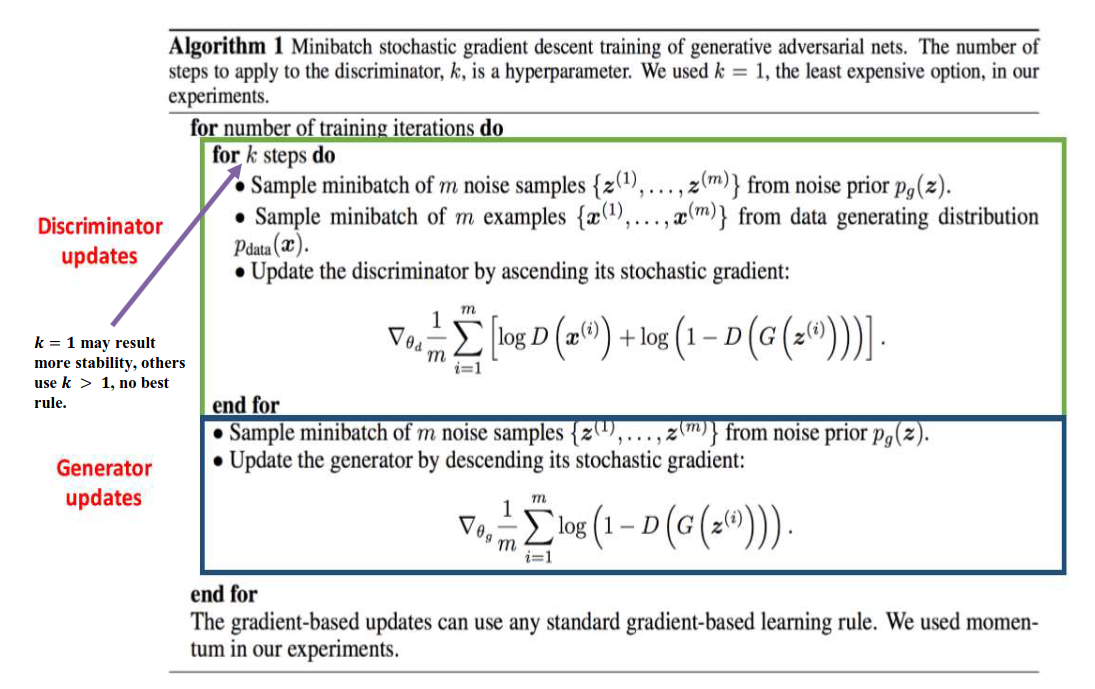
\includegraphics[scale=0.4]{img/09_GAN/alternative_gd.png}
  \end{center}
  It is usually the case that the generator does better than the disciminator, so we sometimes make $k > 1$ to allow more steps for training. 

  There is a vanishing gradient problem in GANs. For instance, assume that the model $\mathcal{G}_{\theta_g}$ has very bad parameters, and it generates very bad samples that the disciminator can detect very well. Then, $\mathbb{E}_{\mathbf{z}} \big[ \log \big( 1 - \mathcal{D}_{\theta_d} (\mathcal{G}_{\theta_g}))\big) \big]$ will be very close to $0$, and the generator's cost will be very flat. Therefore, the gradient would die out and the generator can't improve! For example, if $\mathcal{D}$ was just a sigmoid function, then we can approximate the gradient of the expectation with a sample of the gradient, which would die out. 
  \begin{align*} 
      \nabla_{\theta_g} V(\mathcal{D}, \mathcal{G}) & = \nabla_{\theta_g} \mathbb{E}_{z \sim q(\mathbf(\mathbf{z})} \big[ \log \big( 1 - \mathcal{D}(\mathcal{G}(\mathbf{z}))\big) \big] \\
                                                    & \approx \nabla_a \log \big( 1 - \sigma(a)\big) \\
                                                    & = - \frac{\sigma(a) \, \big( 1 - \sigma(a)\big)}{1 - \sigma(a)} = - \sigma(a) = - \mathcal{D}(\mathcal{G}(\mathbf{z})) 
  \end{align*} 
  and so the gradient goes to $0$ if $\mathcal{D}$ is confident, i.e. $\mathcal{D}(\mathcal{G}(\mathbf{z})) \rightarrow 0$. Therefore, we can modify the cost for the generator term by changing the cost to 
  \[\mathbb{E}_{\mathbf{z}} \log \big( 1 - \mathcal{D}_{\theta_d} ( \mathcal{G}_{\theta_g} (\mathbf{z}))\big)\]
  and trying to minimize it. 


  \begin{theorem}[Nash Equilibrium] 
  Given the minimax loss above, for a fixed $\mathcal{G}$, the optimal discriminator $\mathcal{D}_G^\ast$ is given by 
  \[\mathcal{D}_G^\ast (\mathbf{x}) = \frac{p(\mathbf{x} \mid \text{real})}{p(\mathbf{x} \mid \text{real}) + p(\mathbf{x} \mid \text{synthesized})}\]
  Therefore, the global minimum of the training criterion, $\max_{\mathcal{D}} V(\mathcal{D}, \mathcal{G})$ is achieved if and only if 
  \[p(\mathbf{x} \mid \text{real}) = p(\mathbf{x} \mid \text{synthesized})\]
  \begin{center}
      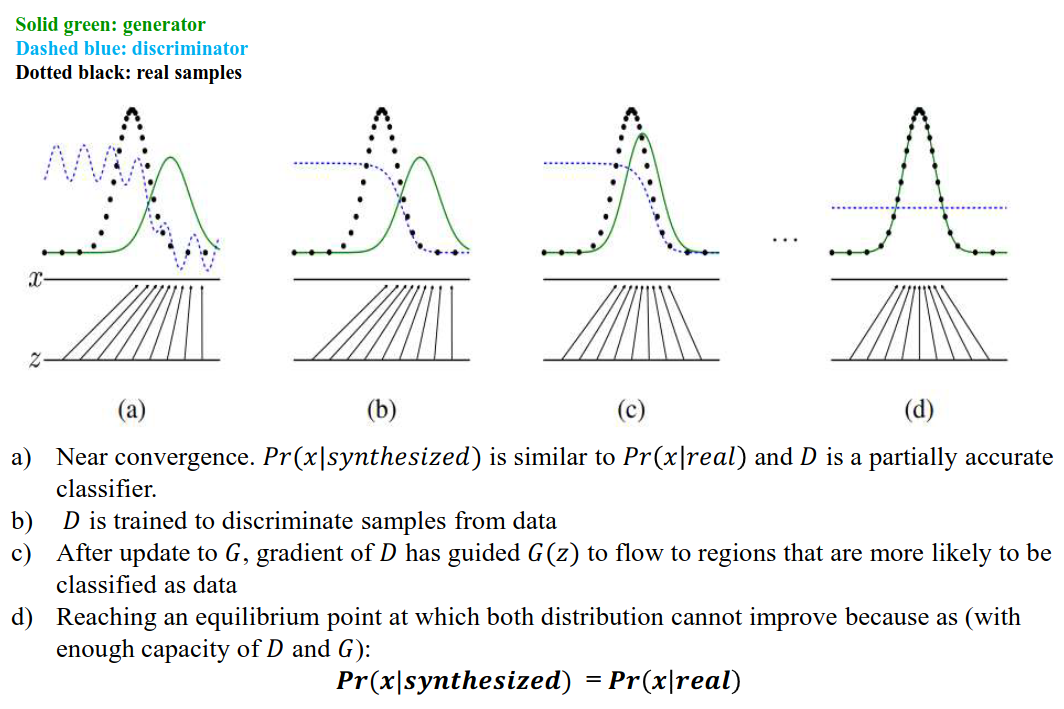
\includegraphics[scale=0.4]{img/09_GAN/nash_equilibrium.png}
  \end{center}
  \end{theorem}
  \begin{proof} 
  We first have 
  \[V(\mathcal{D}, \mathcal{G}) = \mathbb{E}_{\mathbf{x} \sim real} \log \mathcal{D}_{\theta_d} (\mathbf{x}) + \mathbb{E}_{\mathbf{z}} \log \big( 1 - \mathcal{D}_{\theta_d} (\mathcal{G}_{\theta_g} (\mathcal{z}))\big) \]
  Since $\mathcal{G}$ is fixed (i.e. $\theta_g$ is fixed) and acting, we can write the second expectation with respect to the probability measure induced by $\mathcal{G}$.
  \begin{align*} 
  V(\mathcal{D}, \mathcal{G}) & = \mathbb{E}_{\mathbf{x} \sim real} \log \mathcal{D}_{\theta_d} (\mathbf{x}) + \mathbb{E}_{\mathbf{w} \sim \text{fake}} \log \big( 1 - \mathcal{D}_{\theta_d} (\mathbf{w}) \big) \\   
                                  & = \int p(\mathbf{x} \mid \text{real}) \log \mathcal{D}_{\theta_d}(\mathbf{x}) \,d\mathbf{x}+ \int p(\mathbf{x} \mid \text{fake}) \, \log \big( 1 - \mathcal{D}_{\theta_d} (\mathbf{x}) \big) \,d\mathbf{x} 
  \end{align*}
  where the $\mathbf{x}$ in the second integral is a dummy variable. Taking the derivative w.r.t. $\mathbf{x}$ and setting equal to $0$ gives 
  \[p(\mathbf{x} \mid \text{real}) \frac{1}{\mathcal{D}_{\theta_d} (\mathbf{x})} + p(\mathbf{x} \mid \text{fake}) \cdot \frac{-1}{1 - \mathcal{D}_{\theta_d}(\mathbf{x})} = 0\]
  implies that 
  \[\mathcal{D}_{\theta_d}( \mathbf{x}) = \frac{p(\mathbf{x} \mid \text{real})}{p(\mathbf{x} \mid \text{real}) + p(\mathbf{x} \mid \text{fake})}\]
  \end{proof} 


  If the discriminator $\mathcal{D}$ is optimal, then the generator is minimizing the \textbf{Jensen-Shannon divergence} between the real and generated (model distributions). However, $\mathcal{D}$ is not optimal in practice since we have limited computational resources, the loss is non-convex, etc. 

